\documentclass[11pt,twoside,a4paper]{article}
\usepackage{mathtools}
\usepackage{pgf,tikz,pgfplots}
\pgfplotsset{compat=1.15}
\usepackage{mathrsfs}
\usetikzlibrary{arrows}
\usepackage{float}
\floatstyle{boxed}
\restylefloat{figure}
\begin{document}
\title{Complex Fourier Series}
\author{Hannah Ellis}
\date{June 2017}
\maketitle
\section{"The Series"}
For a function $f(x)$ with range $-\frac{a}{2}<x<\frac{a}{2}$ we assume that it can
be reproduced by a sum of complex exponentials of the form
\begin{equation}
exp(i k_n x)
\end{equation}

Where $k=\frac{2n\pi}{a}$ so that n periods of a complex exponential fit's into
the range $-\frac{a}{2}<x<\frac{a}{2}$. Along with complex coefficients for each
term, we get the equation

\begin{equation}
\label{eq:cfs}
f(x)=\sum_{n=-infty}^{infty} c_n \exp\left(\frac{2ni\pi}{a}x\right)
\end{equation}
This is the complex Fourier series.

\section{"An interesting result"}
To calculate any particular coefficient, it will be important to evaluate the
following intergral.
\begin{subequations}
\begin{align}
I_{nm} &=int_{-\frac{a}{2}}^{\frac{a}{2}} \exp \left( \frac{2 i n \pi}{a} x\right) \exp \left( \frac{-2 i m \pi}{a} x\right) dx \\
       &=int_{-\frac{a}{2}}^{\frac{a}{2}} \exp \left( \frac{2 i (n - m ) \pi}{a} x\right) dx
\end{align}
letting $p=(n-m)$
\begin{align}
I_{nm}  &=int_{-\frac{a}{2}}^{\frac{a}{2}} \exp \left( \frac{2 i p \pi}{a} x\right) dx \\
        &=\frac{a}{2 i p \pi} \left[\exp \left( \frac{2 i p \pi}{a} x\right)\right]_{-\frac{a}{2}}^{\frac{a}{2}} \\
        &=\frac{a}{2 i p \pi} \left[\exp \left( \frac{2 i p \pi}{a} \frac{a}{2}\right) - \exp \left( -\frac{2 i p \pi}{a} \frac{a}{2}\right)\right]\\
        &=\frac{a}{2 i p \pi} \left[\exp \left( i p \pi \right) - \exp \left(  - i p \pi \right)\right]
\end{align}
using $\exp(ix) = \cos(x) + i \sin(x)$
\begin{align}
I_{nm}  &=\frac{a}{2 i p \pi} \left[\cos(p\pi) + i \sin(p\pi) - \left(\cos(p\pi) - i \sin(p\pi)\right)\right]\\
        &=\frac{a}{2 i p \pi} \left[\cos(p\pi) + i \sin(p\pi) - \cos(p\pi)  + i \sin(p\pi)\right]\\
        &=\frac{a}{2 i p \pi} \left[2i \sin(p\pi) \right]\\
        &=\frac{a}{p \pi} \sin(p\pi)\\
        &=a \frac{\sin(p\pi)}{p\pi}\\
        &=a \text{sinc}(p\pi)
\end{align}
\end{subequations}

\begin{figure}[h]
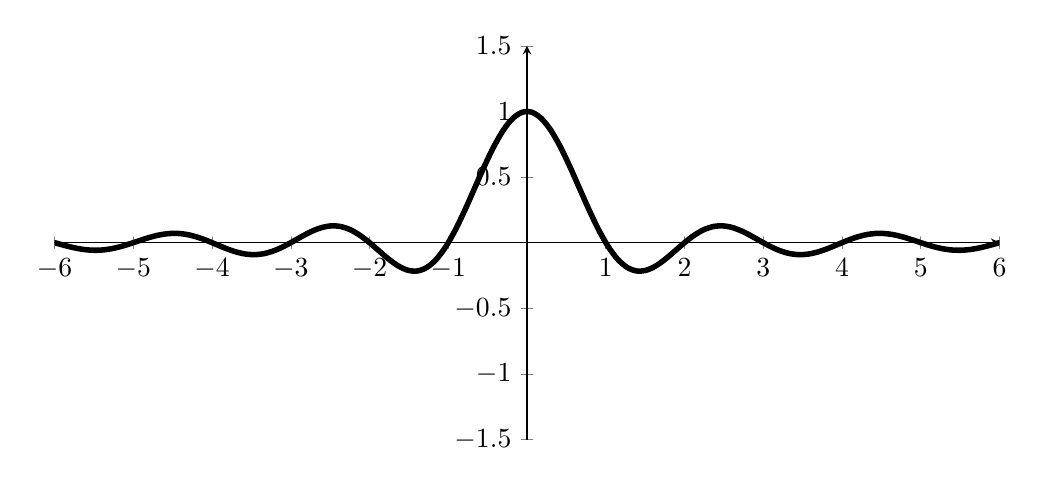
\begin{tikzpicture}[line cap=round,line join=round,>=triangle 45,x=1.0cm,y=1.6666666666666665cm]
\begin{axis}[
x=1.0cm,y=1.6666666666666665cm,
axis lines=middle,
xmin=-6.000000000000001,
xmax=6.0,
ymin=-1.5000000000000002,
ymax=1.5000000000000002,
xtick={-6.0,-5.0,...,6.0},
ytick={-1.5,-1.0,...,1.5},]
\clip(-6.,-1.5) rectangle (6.,1.5);
\draw[line width=2.pt,smooth,samples=100,domain=-6.000000000000001:6.0] plot(\x,{sin(((\x)*3.141592653589793)*180/pi)/((\x)*3.141592653589793)});
\end{axis}
\end{tikzpicture}
\caption{plot of $\text{sinc}(x\pi)$}
\end{figure}

\end{document}
